\section{xmltree Class Reference}
\label{classxmltree}\index{xmltree@{xmltree}}
{\tt \#include $<$xmltree.h$>$}

\subsection*{Public Member Functions}
\begin{CompactItemize}
\item 
{\bf xmltree} (void)
\item 
{\bf $\sim$xmltree} (void)
\item 
bool {\bf load} (QString xmlfile)
\end{CompactItemize}
\subsection*{Public Attributes}
\begin{CompactItemize}
\item 
QDom\-Document {\bf dommodel}
\end{CompactItemize}


\subsection{Detailed Description}




Definition at line 8 of file xmltree.h.

\subsection{Constructor \& Destructor Documentation}
\index{xmltree@{xmltree}!xmltree@{xmltree}}
\index{xmltree@{xmltree}!xmltree@{xmltree}}
\subsubsection{\setlength{\rightskip}{0pt plus 5cm}xmltree::xmltree (void)}\label{classxmltree_17a7ee598a19c132e65454eb12c81c43}




Definition at line 9 of file xmltree.cpp.\index{xmltree@{xmltree}!~xmltree@{$\sim$xmltree}}
\index{~xmltree@{$\sim$xmltree}!xmltree@{xmltree}}
\subsubsection{\setlength{\rightskip}{0pt plus 5cm}xmltree::$\sim$xmltree (void)}\label{classxmltree_8194144c9bea144ab12c218d97bc1350}




Definition at line 14 of file xmltree.cpp.

\subsection{Member Function Documentation}
\index{xmltree@{xmltree}!load@{load}}
\index{load@{load}!xmltree@{xmltree}}
\subsubsection{\setlength{\rightskip}{0pt plus 5cm}bool xmltree::load (QString {\em xmlfile})}\label{classxmltree_40ceaaf2da01e919f0735ad703356e49}




Definition at line 19 of file xmltree.cpp.

References dommodel.

Referenced by treescreen::init\_\-knowtree().

Here is the caller graph for this function:\begin{figure}[H]
\begin{center}
\leavevmode
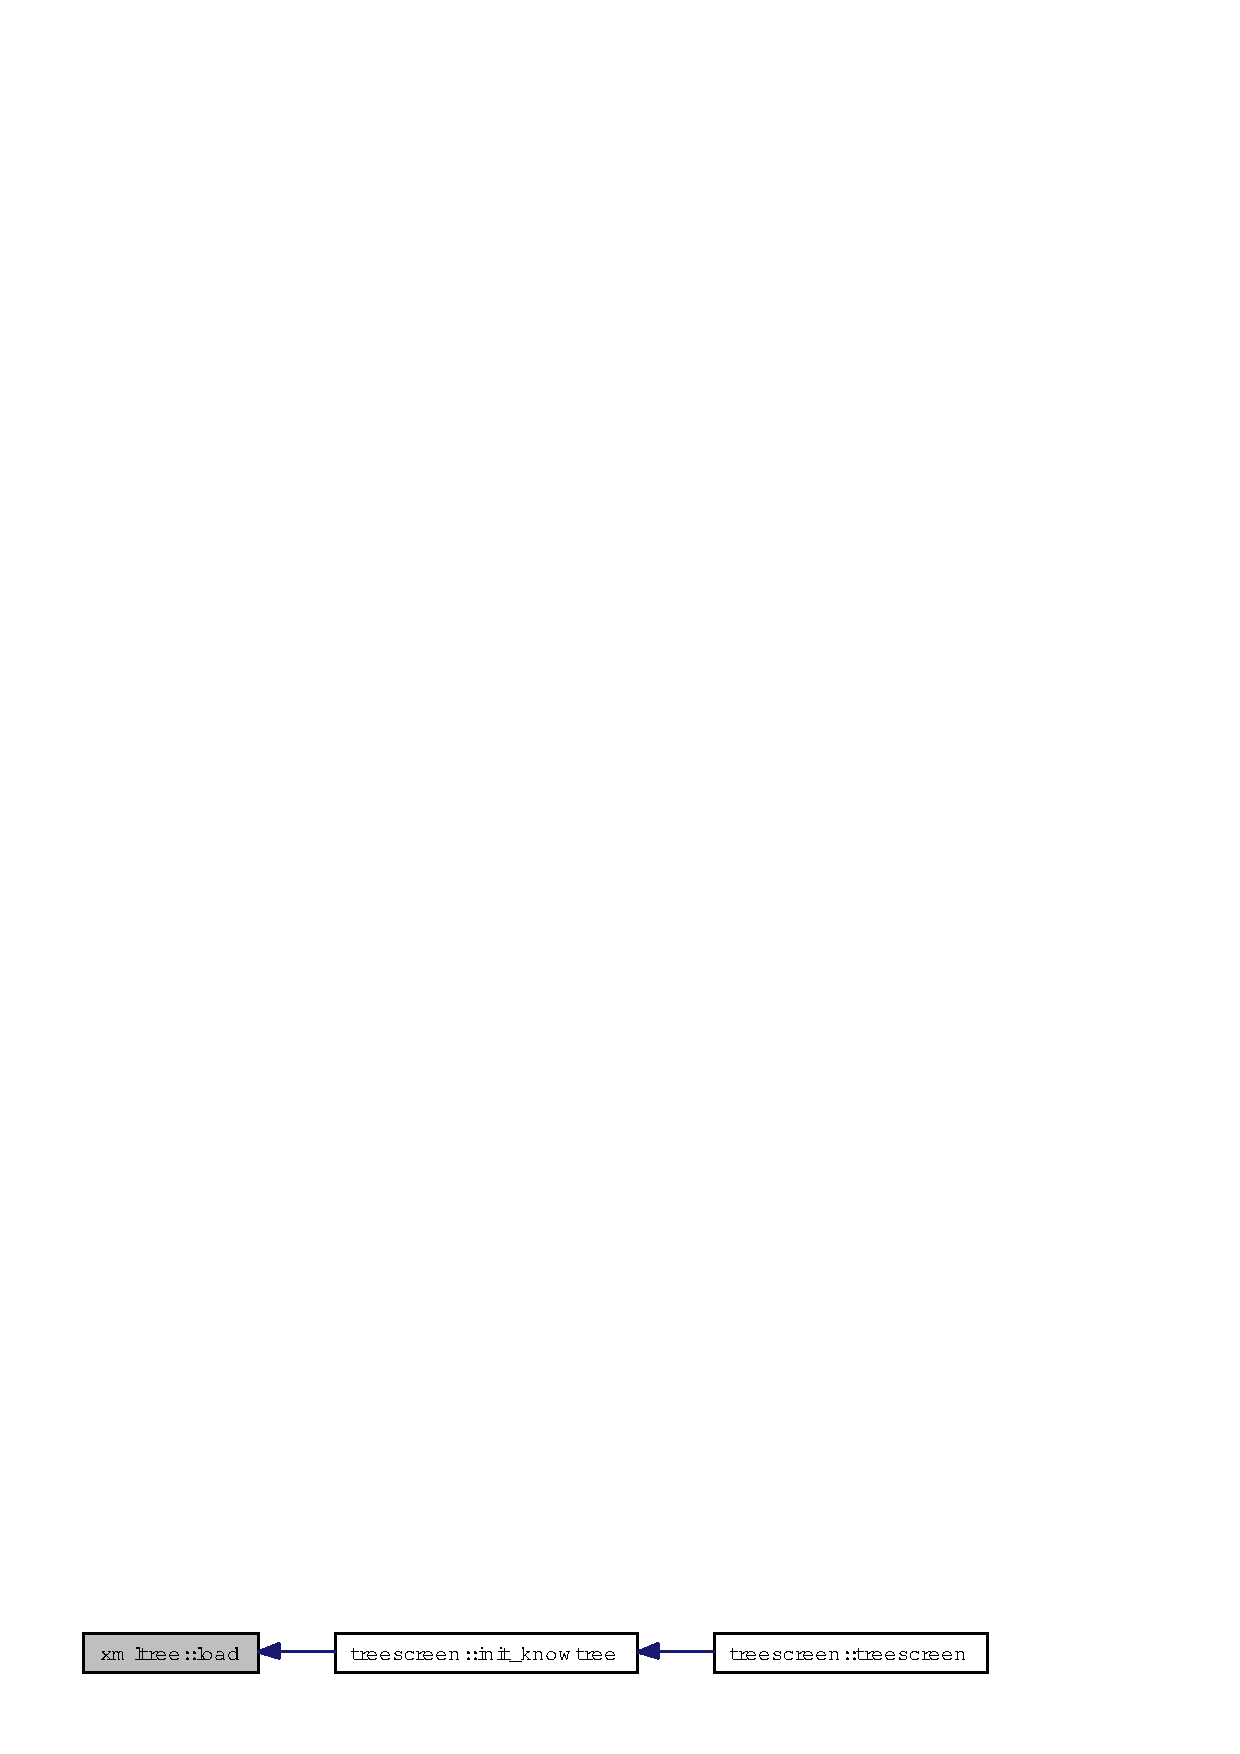
\includegraphics[width=239pt]{classxmltree_40ceaaf2da01e919f0735ad703356e49_icgraph}
\end{center}
\end{figure}


\subsection{Member Data Documentation}
\index{xmltree@{xmltree}!dommodel@{dommodel}}
\index{dommodel@{dommodel}!xmltree@{xmltree}}
\subsubsection{\setlength{\rightskip}{0pt plus 5cm}QDom\-Document {\bf xmltree::dommodel}}\label{classxmltree_6b469b6c9de2ec31c4ba1c8444ba5994}




Definition at line 17 of file xmltree.h.

Referenced by treescreen::init\_\-knowtree(), and load().

The documentation for this class was generated from the following files:\begin{CompactItemize}
\item 
{\bf xmltree.h}\item 
{\bf xmltree.cpp}\end{CompactItemize}
